%%
\documentclass[%
]{ittmm}


\usepackage{tikz}
\usetikzlibrary{positioning}


%%% One can fix some overfulls
\sloppy

%% Minted listings support
%% Need pygment <http://pygments.org/> <http://pypi.python.org/pypi/Pygments>
\usepackage{minted}
%% auto break lines
\setminted{breaklines=true}

%% end of the preamble, start of the body of the document source.
\begin{document}

%%
%% Rights management information.
%% CC-BY is default license.
\copyrightyear{2025}
\copyrightclause{Copyright for this paper by its authors.
  Use permitted under Creative Commons License Attribution 4.0
  International (CC BY 4.0).}

%%
%% This command is for the conference information
\conference{Information and Telecommunication Technologies and Mathematical Modeling of High-Tech Systems 2025 (ITTMM 2025), Moscow, April 07--11, 2025}

%%
%% The "title" command
\title{Application of Neural Network Approach to Numerical Integration}

%%
%% The "author" command and its associated commands are used to define
%% the authors and their affiliations.
\author[1]{Gregory A. Shipunov}[%
orcid=0009-0007-7819-641X,
email=shgregory3@gmail.com,
]
\cormark[1]

\author[1,2]{Oksana I. Streltsova}[%
orcid=0000-0003-4522-6735,
email=strel@jinr.ru,
]

\author[1,2]{Yuriy L. Kalinovskiy}[%
orcid=0000-0002-7596-5531,
email=kalinov@jinr.ru,
]
\address[1]{Dubna State University,
  19 Universitetskaya St, Dubna, 141980, Russian Federation}
\address[2]{Joint Institute for Nuclear Research,
  6 Joliot-Curie St, Dubna, 141980, Russian Federation}

%%% Footnotes
\cortext[1]{Corresponding author.}

%% The abstract is a short summary of the work to be presented in the
%% article.
\begin{abstract}
    This paper is dedicated to the description of the application of neural network approach to numerical integration of functions of one and multiple variables. The essence of the approach is to train a neural network model to approximate the integral function and than use the parameters of the model to numerically calculate the value of the integral using the formulae based on those parameters. The usage of the approach will reduce the amount of calculations (and time) required to get a numerical integration result when the number of integral function's variables is big. Where the common numerical methods become too complex, the numerical approach allows calculations to be less demanding of the computational time and resources. This approach is being tested within the framework of a physics problem of modeling of the particles formation and their properties in the NICA experiment. In this experiment the key problem is to calculate integrals of functions of multiple variables. Currently the author of this paper is developing the framework for integration of functions of two variables. The main goal of the project though is to develop a Python library for numerical integration based on neural network approach.

\end{abstract}

%% Keywords. The author(s) should pick words that accurately describe
%% the work being presented. Separate the keywords with commas.
\begin{keywords}
  neural networks \sep
  numerical integration \sep
  meson \sep
  NICA \sep
  python library
\end{keywords}

%% This command processes the author and affiliation and title
%% information and builds the first part of the formatted document.
\maketitle

\section{Introduction}

The problem of numerical integration appears in both theoretical and applied calculations and potentially raises two obstacles. The first one is the complexity of the analytical form of the anti-derivative of the integral function (which is required to get the value of the definite integral). Sometimes it is just hard to produce the anti-derivative of the function and sometimes there are none. In general case there is no general algorithm to get a given function's anti-derivative. Methods of numerical integration exist (e.g. Simpson's method) to solve this problem by providing a formulae to get the value of an integral with some error without knowing the anti-derivative. But as the dimensions of the integral function's grow, the complexity of those methods also grows as well as the error bound. In this case the neural network approach to the numerical integration may help reduce the complexity as well as increase accuracy of the calculation.

Currently, there were several works done in the field of application of neural networks to the numerical integration problem. We here will highlight the paper "Using neural networks for fast numerical integration and optimization" by Lloyd et al.\cite{lloyd2020using}. This work was served as an inspiration for the development of the neural network approach. Another source was the physics problem of modeling of the particles formation and their properties in the NICA experiment which involves solving the equations containing double and triple integrals. The development of this neural network approach to the numerical integration has the main goal of the development of a software library for the Python programming language with functionality of numerical integration based on neural network approach.

This paper contains several parts. Firstly, we will give the description of one of the possible neural network approaches to the numerical integration as well as highlight other potential approaches. Secondly, the physics problem of modeling of the of the particles formation and their properties in the NICA experiment will be depicted. Thirdly, we will give the observation on the results already reached in the development of the neural network approach to the numerical integration. Lastly, the insight on the future of this project will be given. 

\section{Neural Network Approach to Numerical Integration}

The problem we are investigating in this paper is the application of neural network approach to the calculation of approximate value of integral of a function, i.e. numerical integral with usage of neural network approach.

Let a continuous real function $f(\mathbf{x})$ be defined as $f: {\rm I\!R}^n \to {\rm I\!R}$. Let $\Omega$ be a compact subset of ${\rm I\!R}^n$ and let $G$ be a bounded convex subset of $\Omega$. Let, also, $\mathbf{x}$ be a vector of $n$ dimensions in $\Omega$. Than

\begin{equation}
    \label{eq: integral definition}
    I(f) = \int_G f(\mathbf{x})d\mathbf{x},
\end{equation}

\noindent is a definite integral of $f$ across set $G$. Therefore, the problem is to get the $I(f)$ value calculated with use of neural network approach.

The work of Lloyd et al.\cite{lloyd2020using} proposes, that function $f(\mathbf{x})$ can be approximated using an MLP (multilayer perceptron) neural network. Let this network contain of 3 layers with sizes $n$, $k$ and $1$ accordingly. $n$ is defined above as a number of dimensions of the function $f(\mathbf{x})$, $k$ is the hidden-layer size which is set to minimize the approximation error and $1$ neuron of the output layer accumulates the approximated $f(\mathbf{x})$ value. Because this value is not equal to the value $f(\mathbf{x})$ with given $\mathbf{x}$, let us denote it as $\hat{f}(\mathbf{x})$ and further on we will refer to the MLP network as $\hat{f}(\mathbf{x})$. Figure \ref{fig:structure} depicts the structure of the $\hat{f}(\mathbf{x})$ network. 

\begin{figure}[h!]
    \centering
    % 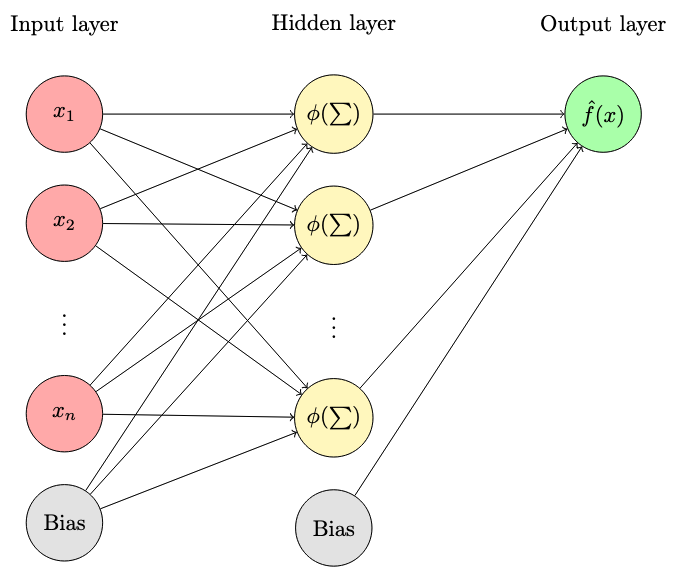
\includegraphics[width=0.6\linewidth]{structure.png}
    % \begin{tikzpicture}[
    %         neuron/.style={circle, draw, minimum size=1.0cm, node distance=1cm},
    %         bias/.style={circle, draw, minimum size=1.0cm, node distance=1cm, fill=gray!20},
    %         layer/.style={draw=none, fill=none}
    %     ]
        
    %     % Input layer
    %     \node[neuron, fill=red!30] (x1) {$x_1$};
    %     \node[neuron, below=0.5cm of x1, fill=red!30] (x2) {$x_2$};
    %     \node[layer, below=0.5cm of x2] (dots1) {$\vdots$};
    %     \node[neuron, below=0.5cm of dots1, fill=red!30 ] (xn) {$x_n$};
    %     \node[bias, below=0.5cm of xn] (b1) {$b^{(1)}$};
        
    %     % Hidden layer
    %     \node[neuron, right=3cm of x1, fill=yellow!30] (h1) {$\phi(\sum)$};
    %     \node[neuron, below=0.5cm of h1, fill=yellow!30] (h2) {$\phi(\sum)$};
    %     \node[layer, below=0.5cm of h2] (dots2) {$\vdots$};
    %     \node[neuron, below=0.5cm of dots2, fill=yellow!30 ] (hK) {$\phi(\sum)$};
    %     \node[bias, below=0.5cm of hK] (b2) {$b^{(2)}$};
        
    %     % Output layer
    %     \node[neuron, right=3cm of h1, fill=green!30] (o) {$\hat{f}(x)$};
        
        
    %     % Connections
    %     \foreach \i in {x1,x2,xn,b1}{
    %         \foreach \j in {h1,h2,hK}{
    %             \draw[->] (\i) -- (\j);
    %         }
    %     }
        
    %     \foreach \i in {h1,h2,hK,b2}{
    %         \draw[->] (\i) -- (o);
    %     }

    %     % Labels
    %     \node[layer, above=0.5cm of x1] {$Input\:layer$};
    %     \node[layer, above=0.5cm of h1] {$Hidden\:layer$};
    %     \node[layer, above=0.5cm of o] {$Output\:layer$};
        
    %     \end{tikzpicture}
    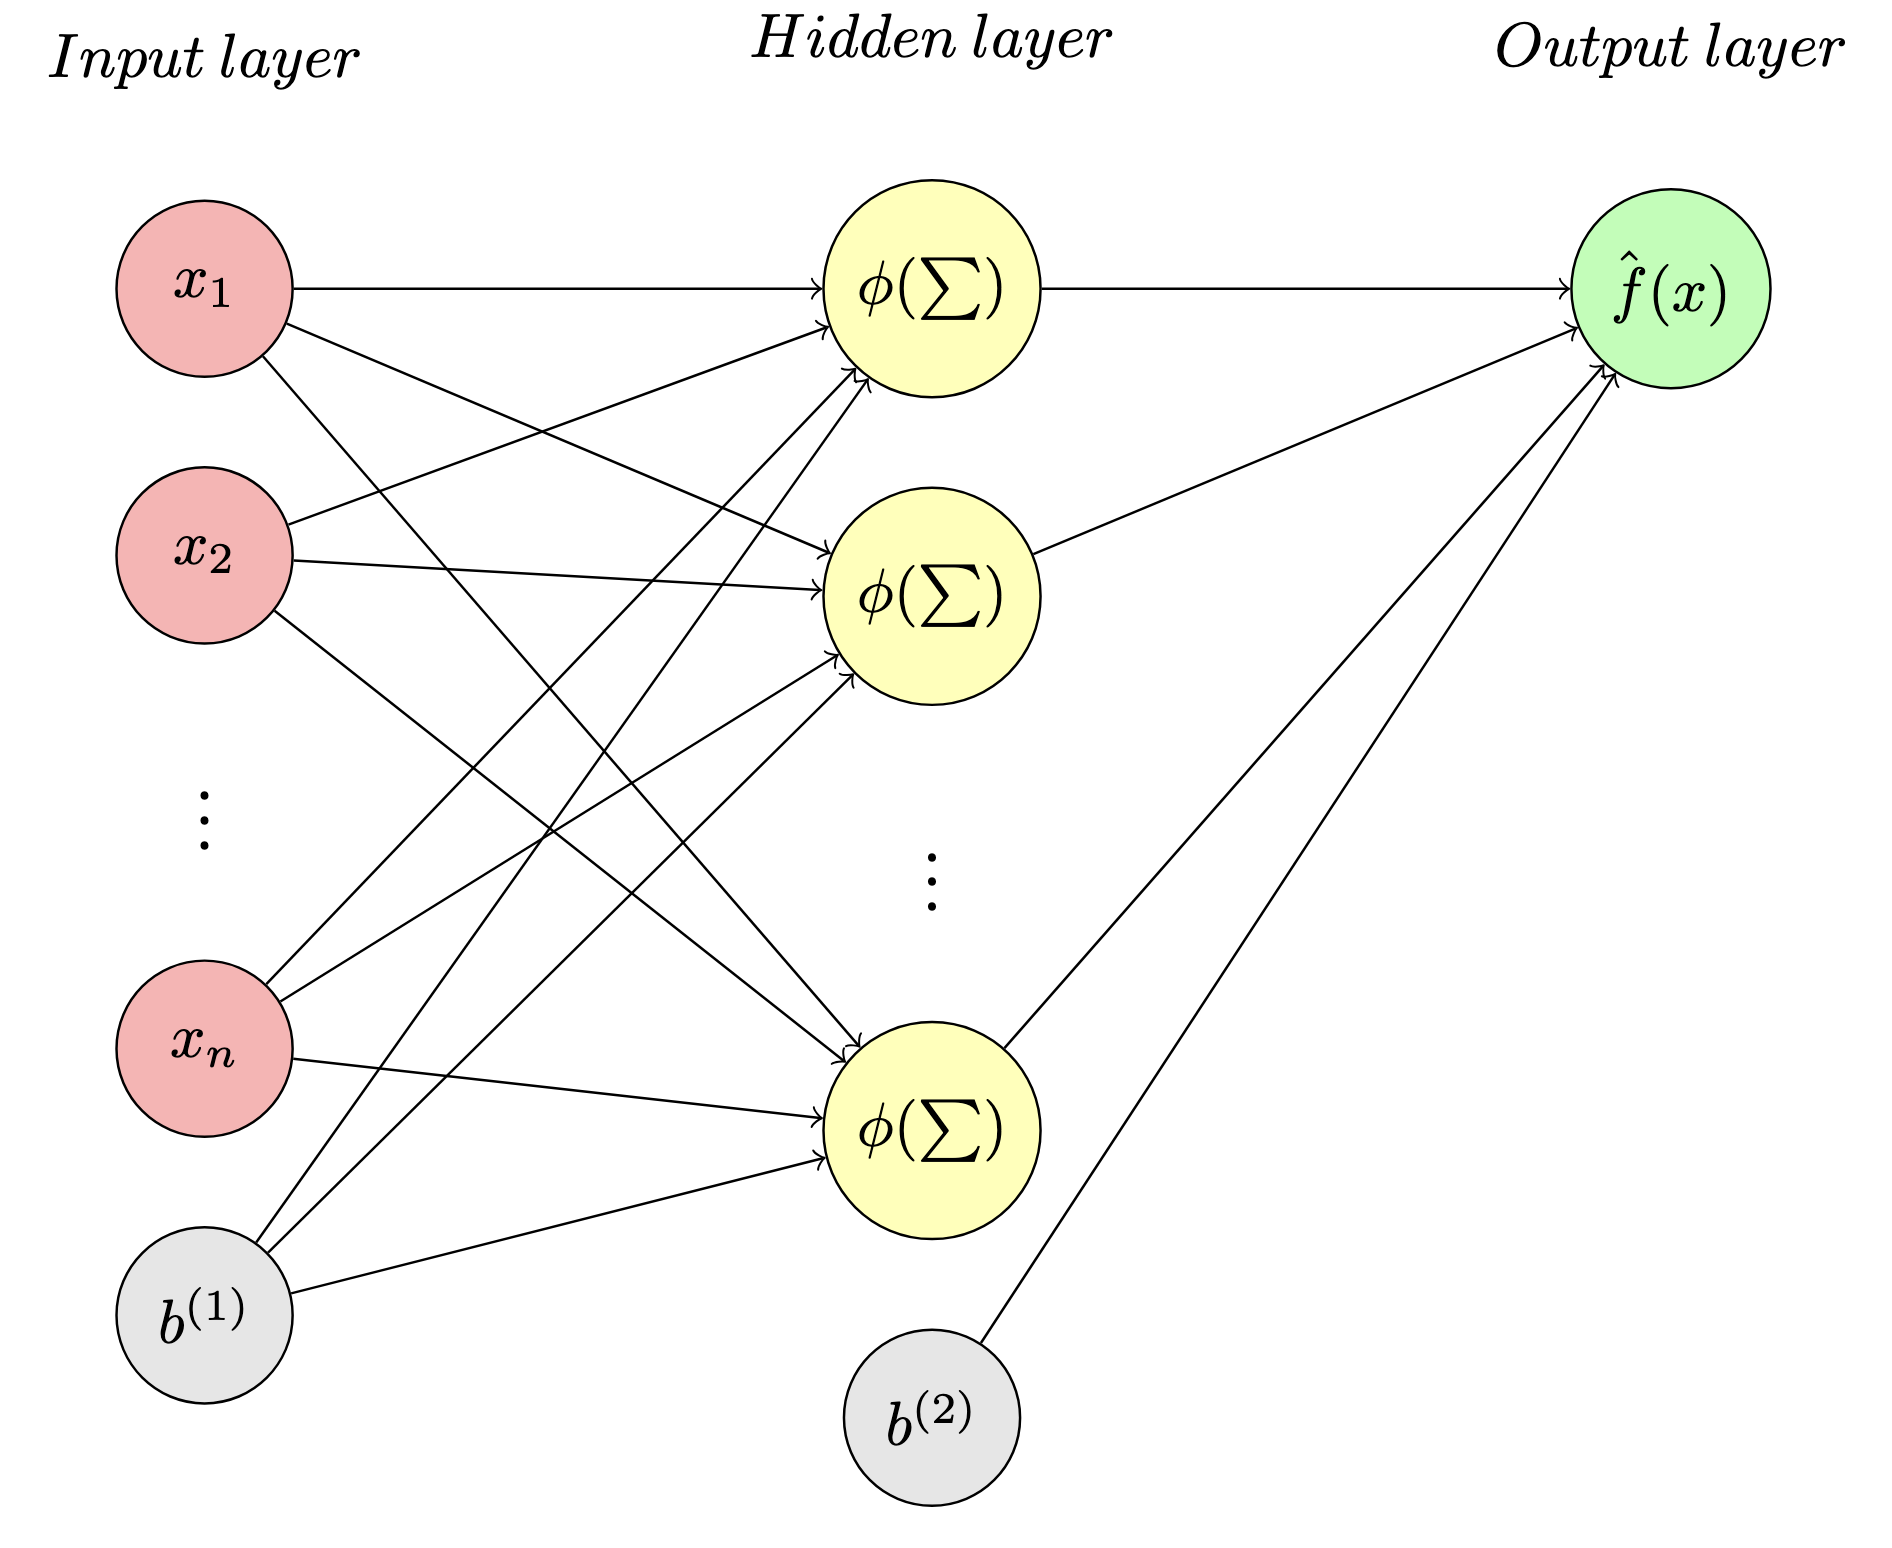
\includegraphics[width=0.4\linewidth]{structre-as-photo.png}
    \caption{The MLP structure used in the neural network approach}
    \label{fig:structure}
\end{figure}

MLP network can have activation functions applied to each neuron's value before this value propagates forward. In our case both input and output layer has \textit{linear activation function} applied and the hidden layer has \textit{logistic sigmoid function} applied. Last has the following definition:

\begin{equation}
    \label{eq:sigmoid}
    \phi(z) = \frac{1}{1+\exp(-z)}.
\end{equation}

\noindent With $\phi(z)$ defined, network structure's mathematical form is:

\begin{equation}
    \label{eq:math-form-mlp}
    \hat{f}(x) = b^{(2)} + \sum_{j=1}^{k}w_j^{(2)}\phi(b_j^{(1)}+\sum_{i=1}^{n}w_{ji}^{(1)}x_{i}).
\end{equation}

So here Lloyd's et al. work puts the proposition to use the trained neural network $\hat{f}(\mathbf{x})$ to get the approximate value of integral (\ref{eq: integral definition}):

\begin{equation}
    \label{eq: ihatdef}
    \hat{I}(f) = \int_G \hat{f}(\mathbf{x})d\mathbf{x}.
\end{equation}

\noindent To integrate the (\ref{eq:math-form-mlp}) and get the value of $\hat{I}(f)$ let us apply following substitution:

\begin{equation}
    \label{eq:substitution-li-sigm}
    -Li_0(-\exp(z)) = \frac{1}{1+\exp(-z)} = \phi(z),
\end{equation}

\noindent where $Li_0(u(z))$ is a Jonquière's function or the polylogarithm of order 0:

\begin{equation}
    \label{eq:li0-def}
    Li_0(u) = \frac{u}{1 - u}.
\end{equation}

\noindent This substitution is proved to be numerically accurate in the Lloyd's et al. work\cite{lloyd2020using}. With substitution (\ref{eq:substitution-li-sigm}) network (\ref{eq:math-form-mlp}) can be integrated over given $G: [\alpha_1, \beta_1] \times...\times[\alpha_n, \beta_n]$ in ${\rm I\!R}^n$. to produce the following numerical integration formulae:

\begin{equation}
        \label{eq:numerical_method_1}
            \hat{I}(f) = b^{(2)}\prod_{i=1}^{n}(\beta_i - \alpha_i) + \sum_{j=1}^{k}w_j^{(2)}[\prod_{i=1}^{n}(\beta_i - \alpha_i) + \frac{\Phi_j}{\prod_{i=1}^{n}w_{ij}^{(1)}}],
        \end{equation}
        \begin{equation}
        \label{eq:numerical_method_2}
            \Phi_j = \sum_{r=1}^{2^n}\xi_{r}Li_n(-exp[-b_j^{(1)} - \sum_{i=1}^{n}w_{ij}^{(1)}l_{i,r}]),
        \end{equation}
        \begin{equation}
        \label{eq:numerical_method_3}
            \xi_{r} = \prod_{d=1}^{n}(-1)^{[{r}/{2^{n-d}}]},
        \end{equation}
        \begin{equation}
        \label{eq:numerical_method_4}
            l_{i,r} = \left\{
            \begin{array}{ll}
                \alpha_i, & \text{if } [{r}/{2^{n-d}}] \% 2 = 0 \\
                \beta_i, & \text{if } [{r}/{2^{n-d}}] \% 2 \neq 0,
            \end{array}
        \right.
\end{equation}
    where $b^{(1)}, b^{(2)}, w^{(1)}, w^{(2)}$ -- neural network's parameters, $\alpha_i, \beta_i, 1 \leq i \leq n$ -- integration boundaries for each dimension, $n$ -- number of $ f(x) $ dimensions.

The described neural network approach to numerical integration concludes to following steps:

\begin{enumerate}
    \item generate the dataset to train, validate and test the neural network model (\ref{eq:math-form-mlp}) to approximate given integral function;
    \item train, validate and test (\ref{eq:math-form-mlp}) to approximate given integral function;
    \item extract parameters of the network (\ref{eq:math-form-mlp}) and use them with (\ref{eq:numerical_method_1}-\ref{eq:numerical_method_4}) to calculate the numerical integral.
\end{enumerate}

\section{Modeling of the  formation of particles and their properties for the NICA experiment}

The main task is to build a model for the unified description of both light and heavy mesons formed in heavy ion collisions.

 This will be a nonlocal interaction model \cite{blaschke, costa}. 
 The model concludes to the fact that meson (quark-antiquark pair) formation proceeds with a gluon exchange. But the gluon exchange cannot be described as a diagram sum, because perturbation theory cannot be applied here. 
 
 Mesons can be described as $q\bar{q}$ bound states by 
the Bethe-Salpeter equation

\begin{eqnarray}\label{BS}
  \Gamma (q,P) = -\frac{4}{3} \int \frac{d^4 p}{(2\pi)^4}
  D(q-p) \gamma_\alpha S_1 \Gamma (q,P)
S_2 \gamma_\alpha \  .
\end{eqnarray}

The vertex function $\Gamma (p,P)$ depends on the relative
momentum $p$, and the total momentum of the bound state $P$. 
$S_i(p)$ are the dressed quark propagator in the Euclidean space 
\begin{equation}\label{Eqn:q_prop}
S_i(p_i)=\frac{1}{i (p_i\cdot \gamma) + m_i}
\end{equation}
The momenta $p_i=p+q_i$, $q_i = b_i P$, $i=1,2$ with 
$b_1 =- m_1/(m_1+m_2)$, $b_2 = m_2/(m_1+m_2)$, $m_i$ are the constituent quark masses. 

Equation (\ref{BS}) contains the interaction kernel $D(q-p)$ 
which describes the effective gluon interaction within a meson. 
We consider the rank -1 separable  model 
\begin{eqnarray}\label{kernel}
  D(q-p) = D_0 F(q^2) F(p^2) \, ,
\end{eqnarray}
where $D_0$ is the coupling constant and the function 
$F(p^2)$ is related to scalar part of Bethe - Salpeter  vertex
function. We employ  $F(q^2)$  in the Gaussian form 
$F(p^2)= e^{-p^2/\lambda^2}$ with the parameter $\lambda$ which  characterizes the finite size of the meson. 

This separable Anzatz of the interaction kernel (\ref{kernel}) allows to write the meson observables in the term of the polarization operator (the buble diagram): 

%\begin{equation}
%    \label{eq:formfactorsize}
%    F(p^2)=\exp\left(\frac{-p^2}{\lambda^2}\right),
%\end{equation}

%\noindent so the form-factor size will be defined by the $F(p^2)$ %as shown above (\ref{eq:formfactorsize}). To describe the particles %we need to know masses, decay constants and the decay process. Let %us denote the interaction diagram as \tikz[baseline=-0.5ex]{
%        \filldraw (0, 0) circle (0.1cm);
%        \filldraw (1, 0) circle (0.1cm);
%        \draw[->, thick] (0.1, 0.05) to[out=45, in=135] (0.9, %0.05);
%        \draw[<-, thick] (0.1, -0.05) to[out=-45, in=-135] (0.9, %-0.05);
%    } and than we can use it in the equations:

\begin{equation}
        \tikz[baseline=-0.5ex]{
        \filldraw (0, 0) circle (0.1cm);
        \filldraw (1, 0) circle (0.1cm);
        \draw[->, thick] (0.1, 0.05) to[out=45, in=135] (0.9, 0.05);
        \draw[<-, thick] (0.1, -0.05) to[out=-45, in=-135] (0.9, -0.05);
    } + \tikz[baseline=-0.5ex]{
        \filldraw (0, 0) circle (0.1cm);
        \filldraw (1, 0) circle (0.1cm);
        \draw[->, thick] (0.1, 0.05) to[out=45, in=135] (0.9, 0.05);
        \draw[<-, thick] (0.1, -0.05) to[out=-45, in=-135] (0.9, -0.05);
    }\tikz[baseline=-0.5ex]{
        \filldraw (0, 0) circle (0.1cm);
        \filldraw (1, 0) circle (0.1cm);
        \draw[->, thick] (0.1, 0.05) to[out=45, in=135] (0.9, 0.05);
        \draw[<-, thick] (0.1, -0.05) to[out=-45, in=-135] (0.9, -0.05);
    } + ... = \frac{1}{1 - \tikz[baseline=-0.5ex]{
        \filldraw (0, 0) circle (0.1cm);
        \filldraw (1, 0) circle (0.1cm);
        \draw[->, thick] (0.1, 0.05) to[out=45, in=135] (0.9, 0.05);
        \draw[<-, thick] (0.1, -0.05) to[out=-45, in=-135] (0.9, -0.05);
    }},
\end{equation}
where 
\begin{equation}
        \tikz[baseline=-0.5ex]{
        \filldraw (0, 0) circle (0.1cm);
        \filldraw (1, 0) circle (0.1cm);
        \draw[->, thick] (0.1, 0.05) to[out=45, in=135] (0.9, 0.05);
        \draw[<-, thick] (0.1, -0.05) to[out=-45, in=-135] (0.9, -0.05);
    } \to \int_{0}^{\infty}\frac{dp}{2\pi^4}F(p^2)\frac{1}{u_1u_2} = \int_{0}^{\infty}\frac{dp}{2\pi^4}F(p^2)\frac{1}{[(p + q_1)^2 + m_1^2][(p + q_2)^2 + m_2^2]}.
\end{equation}

To calculate these integrals we use the equations:

\begin{equation}
    \frac{1}{(p + q_i)^2 + m_i^2} = \int_{0}^{\infty}dt\{\exp(-t[(p + q_i)^2 + m_i^2])\}, 
\end{equation}
\begin{equation}
    F(p^2) = \int_{0}^{\infty}ds\{\exp(-sp^2)F(s)\} .
\end{equation}

The case of more than two mesons is described using triple and quadruple integrals.

The amplitudes of particular decays and the squared amplitudes of particular decays are calculated using FORM 
(software for analytical calculation). But the key problem is to calculate integrals of functions of multiple variables.

In the framework of this problem there is a particular iterated integral:

\begin{equation}
    \label{eq:the-integral}
    \int_{0}^{1}d\alpha\{\alpha^{a}(1 - \alpha)^b\}\int_{0}^{\infty}dt\{\frac{t^m}{(1+t)^n}F[z_{0}]\} \equiv I(a, b, m, n; F[z_{0}]),
\end{equation}
\begin{equation}   
    F[z_0] = \exp[-2z_0],
\end{equation}
\begin{equation} 
    z_0 = tD + \frac{t}{1 + t}R^2,
\end{equation}
\begin{equation}     
    D = \alpha_1(b_1^{2}P^2 + m_1^2) + \alpha_2(b_2^{2}P^2 + m_2^2),
\end{equation}
\begin{equation} 
        R^2 = (\alpha_1^{2}b_1^2 + \alpha_2^{2}b_2^2 + 2\alpha_{1}\alpha_{2}b_{1}b_2)P^2,
\end{equation}
\begin{equation} 
    b_1 = -\frac{m_1}{m_1 + m_2},
\end{equation}
\begin{equation} 
    b_2 = \frac{m_2}{m_1 + m_2},
\end{equation}
\begin{equation}
    \alpha_1 = \alpha, \alpha_2 = 1 - \alpha.
\end{equation}

\begin{figure}
    \centering
    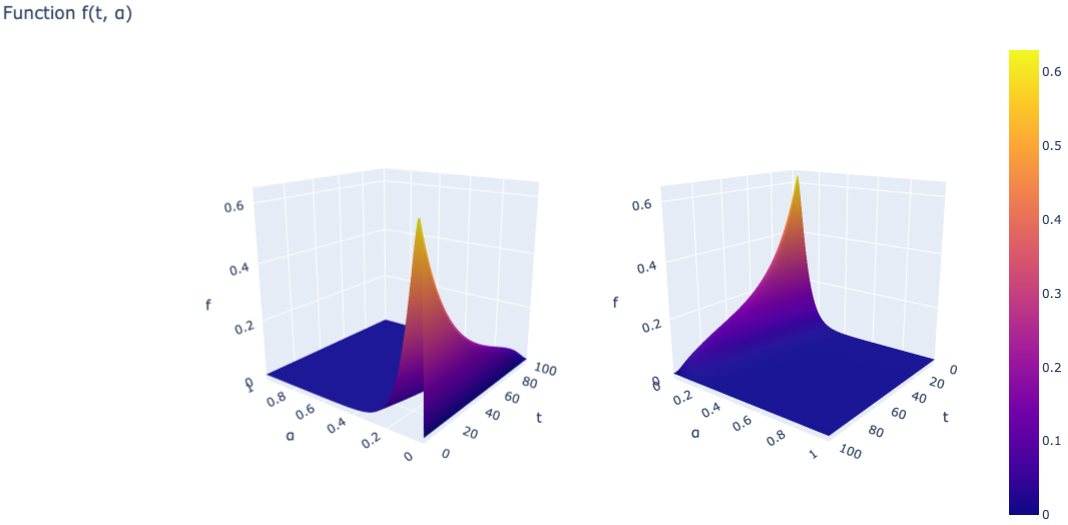
\includegraphics[width=0.8\linewidth]{f(t,a)33.png}
    \caption{Integrand function (\ref{eq:the-integral}) plot - view from (0, 0, 0) and (100, 0, 0) corners}
    \label{fig:integrand-plot}
\end{figure}

\noindent This integral is used in multiple calculations in the problem. Shape of its 2-dimensional integral is sown on Figure 2. As it can be seen in (\ref{eq:the-integral}) it is denoted as $I(a, b, m, n; F[z_{0}])$, and with different combination of parameters it is used multiple times in the calculations. The integral (\ref{eq:the-integral}) also is interesting in that case, that it depends on two variables only, so it is can be used to test the integration framework we've been developing early in the development cycle. 

\section{Approach testing}

TEXT

\section{Usage of Neural Network Approach}

As stated in the previous part, the integral (\ref{eq:the-integral}) has been already used to test the neural network approach. 

It was firstly interpreted as a product of two integrals of single-variable functions ($\alpha_{1,2}$ were treated as constants). The first integral of function $\alpha^{a}(1 - \alpha)^b$ has a very simple analytical anti-derivative with any integer parameter $a$ and $b$ so it was easy to check the result of the integration. In most cases the neural network approach provided error bound $\varepsilon < 10^{-5}$. On the other hand, the second integral of function $\frac{t^m}{(1+t)^n}F[z_{0}]$ has a much more complex anti-derivative, so in this case the goal was to make the approximation bound of neural network $\hat{f}(x)$ was $\epsilon < 10^{-5}$ and this requirement was met.

Secondly, the iterated integral (\ref{eq:the-integral}) was interpreted as a double integral:

\begin{equation}
    \label{eq:iterated-as-double}
     \int_{0}^{1} \alpha^{a}(1 - \alpha)^bd\alpha \int_{0}^{\infty}\frac{t^m}{(1+t)^n}F[z_{0}]dt = 
     \int_{0}^{1} \int_{0}^{\infty}\frac{t^m}{(1+t)^n}F[z_{0}]\alpha^{a}(1 - \alpha)^bdtd\alpha ,
\end{equation}

\noindent and this double integral function was used to train the neural network model to approximate it. The approximation error bound of $\epsilon < 10^{-5}$ was also met, but currently the software implementation of the formulae (\ref{eq:numerical_method_1}-\ref{eq:numerical_method_4}) requires further improvement and testing.

Also both 1-dimensional ans 2-dimensional functionality was tested on simple arbitrary functions, e.g. transcendental functions.

\section{Future development}

Currently, the further development of the neural network approach to the numerical integration continues. The resulting software will be tested on the integrals from the meson interaction modeling problem, which provides plenty of cases where numerical integration of high-dimensional functions is required. Also, we hope, the final product - the software library for numerical integration with use of numerical integration approach called \textit{Skuld} will help to solve difficult calculation problems in the meson interaction modeling problem domain as well, as in other fields, both theoretical and applied.

\section{Acknowledgments}

Authors of this work express their acknowledgments to Sara Shadmehri and Tatevik Bezhanyan from Meshcheryakov Laboratory of Information Technologies, JINR for their advices both in the field of neural networks and English language.

\bibliography{main}

\end{document}
